%Translate this Latex book chapter to Spanish. Output in Latex format. Rearrange bullet points (\items) into full paragraphs. Make sure that sentences are connected in a more fluid way as they come. Elaborate on incomplete ideas where appropriate.

\section{Tareas de Etiquetado de Secuencias o Etiquetado}
\begin{itemize}
  \item El etiquetado de secuencias o etiquetado es una tarea en PNL que difiere de la clasificación de documentos.
  \item El objetivo es asignar etiquetas o etiquetas a una oración representada como una secuencia de tokens $x_1, x_2, \dots, x_n$.
  \item En particular, el objetivo del etiquetado de secuencias es asignar etiquetas a palabras, o más generalmente, asignar etiquetas discretas a elementos discretos en una secuencia \cite{jacobbook}.
  \item Ejemplos conocidos de esta tarea son el etiquetado de partes del discurso (POS) y el reconocimiento de entidades nombradas (NER).
\end{itemize}

\section{Etiquetado de Partes del Discurso}
\textcolor{green}{\textbf{ENTRADA:}}
Los beneficios aumentaron en Boeing Co., superando fácilmente las previsiones en Wall Street, cuando su CEO Alan Mulally anunció los resultados del primer trimestre.  \vspace{0.5cm}

\textcolor{green}{\textbf{SALIDA:}}
Los beneficios\textcolor{red}{/N} aumentaron\textcolor{red}{/V} en\textcolor{red}{/P} Boeing\textcolor{red}{/N} Co.\textcolor{red}{/N} ,\textcolor{red}{/,} superando\textcolor{red}{/V} fácilmente\textcolor{red}{/ADV} las\textcolor{red}{/DET} previsiones\textcolor{red}{/N} en\textcolor{red}{/P} Wall\textcolor{red}{/N} Street\textcolor{red}{/N} ,\textcolor{red}{/,} cuando\textcolor{red}{/P} su\textcolor{red}{/DET} CEO\textcolor{red}{/N} Alan\textcolor{red}{/N} Mulally\textcolor{red}{/N} anunció\textcolor{red}{/V} los\textcolor{red}{/DET} resultados\textcolor{red}{/N} del\textcolor{red}{/PREP} primer\textcolor{red}{/ADJ} trimestre\textcolor{red}{/N} .\textcolor{red}{/.}  \vspace{0.5cm}

\begin{itemize}
  \item \textcolor{red}{N} = \textcolor{blue}{Sustantivo}
  \item \textcolor{red}{V} = \textcolor{blue}{Verbo}
  \item \textcolor{red}{P} = \textcolor{blue}{Preposición}
  \item \textcolor{red}{Adv} = \textcolor{blue}{Adverbio}
  \item \textcolor{red}{Adj} = \textcolor{blue}{Adjetivo}
  \item ...
\end{itemize}

\begin{figure}[h]
  \includegraphics[scale=0.34]{pics/posTags.png}
\end{figure}
Fuente: \cite{JurafskyBook}

\section{Reconocimiento de Entidades Nombradas (NER)}
Una \textbf{entidad nombrada} es, hablando en términos generales, cualquier cosa a la que se puede hacer referencia con un nombre propio: una persona, un lugar, una organización. \vspace{0.5cm}

\textcolor{green}{\textbf{ENTRADA:}}
Los beneficios aumentaron en Boeing Co., superando fácilmente las previsiones en Wall Street, cuando su CEO Alan Mulally anunció los resultados del primer trimestre.  \vspace{0.5cm}

\textcolor{green}{\textbf{SALIDA:}}
Los beneficios aumentaron en \textcolor{red}{[Compañía} Boeing Co.\textcolor{red}{]}, superando fácilmente las previsiones en \textcolor{red}{[Lugar} Wall Street\textcolor{red}{]}, cuando su CEO \textcolor{red}{[Persona} Alan Mulally\textcolor{red}{]} anunció los resultados del primer trimestre. \vspace{0.5cm}

\begin{itemize}
  \item Dado que las entidades pueden abarcar varias palabras (es decir, un problema de reconocimiento de fragmentos), podemos utilizar el etiquetado BIO \cite{ramshaw1999text} para convertir el problema en un problema de etiquetado de secuencias.
  \item Etiquetado BIO: utilizar etiquetas que capturen tanto el límite como el tipo de entidad nombrada.
\end{itemize}

\paragraph{Etiquetado BIO: NER como Etiquetado de Secuencias}
\textcolor{green}{\textbf{ENTRADA:}}
Los beneficios aumentaron en Boeing Co., superando fácilmente las previsiones en Wall Street, cuando su CEO Alan Mulally anunció los resultados del primer trimestre.  \vspace{0.5cm}

\textcolor{green}{\textbf{SALIDA:}}
Los\textcolor{red}{/O} beneficios\textcolor{red}{/O} aumentaron\textcolor{red}{/O} en\textcolor{red}{/O} Boeing\textcolor{purple}{/B-C} Co.\textcolor{purple}{/I-C} ,\textcolor{red}{/O} superando\textcolor{red}{/O} fácilmente\textcolor{red}{/O} las\textcolor{red}{/O} previsiones\textcolor{red}{/O} en\textcolor{red}{/O} Wall\textcolor{purple}{/B-L} Street\textcolor{purple}{/I-L} ,\textcolor{red}{/O} cuando\textcolor{red}{/O} su\textcolor{red}{/O} CEO\textcolor{red}{/O} Alan\textcolor{purple}{/B-P} Mulally\textcolor{purple}{/I-P} anunció\textcolor{red}{/O} los\textcolor{red}{/O} resultados\textcolor{red}{/O} del\textcolor{red}{/O} primer\textcolor{red}{/O} trimestre\textcolor{red}{/O} .\textcolor{red}{/O}  \vspace{0.5cm}

\begin{itemize}
  \item \textcolor{red}{O} = \textcolor{blue}{Fuera (sin entidad)}
  \item \textcolor{purple}{B-C} = \textcolor{blue}{Comienzo de Compañía}
  \item \textcolor{purple}{I-C} = \textcolor{blue}{Dentro de Compañía}
  \item \textcolor{purple}{B-L} = \textcolor{blue}{Comienzo de Lugar}
  \item \textcolor{purple}{I-L} = \textcolor{blue}{Dentro de Lugar}
  \item \textcolor{purple}{B-P} = \textcolor{blue}{Comienzo de Persona}
  \item \textcolor{purple}{I-P} = \textcolor{blue}{Dentro de Persona}
\end{itemize}

Nuestro objetivo:
\textbf{Conjunto de entrenamiento:}
\begin{enumerate}
  \item Pierre\textcolor{red}{/NNP} Vinken\textcolor{red}{/NNP},\textcolor{red}{/,} 61\textcolor{red}{/CD} años\textcolor{red}{/NNS} de edad\textcolor{red}{/JJ},\textcolor{red}{/,} se unirá a la junta directiva como director no ejecutivo el 29 de noviembre.\textcolor{red}{/NNP}
  \item El Sr.\textcolor{red}{/NNP} Vinken\textcolor{red}{/NNP} es presidente\textcolor{red}{/NN} de Elsevier\textcolor{red}{/NNP} N.V.\textcolor{red}{/NNP}, el grupo editorial holandés.\textcolor{red}{/NNP}
  \item Rudolph\textcolor{red}{/NNP} Agnew\textcolor{red}{/NNP},\textcolor{red}{/,} de 55\textcolor{red}{/CD} años\textcolor{red}{/NNS} y presidente\textcolor{red}{/NN} de\ldots
\end{enumerate}

\subsection{Etiquetado de secuencias como aprendizaje supervisado}

\begin{itemize}
  \item Tenemos una secuencia de entradas $x = (x_1, x_2, \ldots, x_n)$ y las etiquetas correspondientes $y = (y_1, y_2, \ldots, y_n)$.
  \item La tarea consiste en aprender una función $f$ que mapea secuencias de entrada a secuencias de etiquetas: $f(x_1,x_2, \ldots, x_n) = y_1, y_2, \ldots, y_n$.
  \item Tenemos un conjunto de entrenamiento de secuencias etiquetadas: $\{(x^{(1)}, y^{(1)}), (x^{(2)}, y^{(2)}), \ldots, (x^{(m)}, y^{(m)})\}$.
\end{itemize}

\subsection{Enfoque generativo para el etiquetado de secuencias}

\begin{itemize}
  \item Los modelos generativos, como el clasificador de Naive Bayes utilizado para clasificación, también se pueden utilizar para tareas de etiquetado de secuencias en PLN.
  \item Enfoque:
  \begin{itemize}
    \item Entrenamiento: Aprender la distribución conjunta $p(x_1,x_2, \ldots, x_n,y_1, y_2, \ldots, y_n)$ de las secuencias de entrada.
    \item Decodificación: Utilizar la distribución aprendida para predecir secuencias de etiquetas para nuevas secuencias de entrada.
  \end{itemize}
  \item La decodificación en el etiquetado de secuencias implica encontrar la secuencia de etiquetas con la mayor probabilidad conjunta: $\arg\max_{y_1, y_2, \ldots, y_n}p(x_1,x_2, \ldots, x_n,y_1, y_2, \ldots, y_n)$.
\end{itemize}

\section{Modelos Ocultos de Markov}

\begin{itemize}
  \item Los Modelos Ocultos de Markov (HMM, por sus siglas en inglés) proporcionan una forma sistemática de manejar problemas de etiquetado de secuencias mediante modelos generativos y algoritmos de decodificación eficientes.
  \item Tenemos una oración de entrada $x = x_1, x_2, \ldots, x_n$ ($x_i$ es la $i$-ésima palabra en la oración).
  \item Tenemos una secuencia de etiquetas $y = y_1, y_2, \ldots, y_n$ ($y_i$ es la $i$-ésima etiqueta en la oración).
  \item Usaremos un HMM para definir $p(x_1, x_2, \ldots, x_n, y_1, y_2, \ldots, y_n)$ para cualquier oración $x_1, \ldots, x_n$ y secuencia de etiquetas $y_1, \ldots, y_n$ de la misma longitud \cite{kupiec1992robust}.
  \item Luego, la secuencia de etiquetas más probable para $x$ es:
  \[
    \arg\max_{y_1,\ldots, y_n} p(x_1, \ldots, x_n, y_1, \ldots, y_n)
  \]
\end{itemize}

\section{Modelos Ocultos de Markov Trigramas (Trigram HMM)}

Para cualquier oración $x_1, \ldots, x_n$ donde $x_i \in V$ para $i = 1, \ldots, n$, y cualquier secuencia de etiquetas $y_1, \ldots, y_{n+1}$ donde $y_i \in S$ para $i = 1, \ldots, n$, y $y_{n+1} = \text{STOP}$, la probabilidad conjunta de la oración y la secuencia de etiquetas es:
\[
  p(x_1, \ldots, x_n, y_1, \ldots, y_{n+1}) = \prod_{i=1}^{n+1} q(y_i | y_{i-2}, y_{i-1}) \prod_{i=1}^{n} e(x_i | y_i)
\]
donde hemos asumido que $x_0 = x_{-1} = *$.

\subsection{Parámetros del modelo}

\begin{itemize}
  \item $q(s|u, v)$ para cualquier $s \in S \cup \{\text{STOP}\}$, $u, v \in S \cup \{*\}$
  \begin{itemize}
    \item El valor de $q(s|u,v)$ se puede interpretar como la probabilidad de ver la etiqueta $s$ inmediatamente después del bigrama de etiquetas $(u, v)$.
  \end{itemize}
  \item $e(x|s)$ para cualquier $s \in S$, $x \in V$ 
  \begin{itemize}
    \item El valor de $e(x|s)$ se puede interpretar como la probabilidad de ver la observación $x$ emparejada con el estado $s$.
  \end{itemize}
\end{itemize}

\paragraph{Un ejemplo}

Si tenemos $n = 3$, $x_1, x_2, x_3$ igual a la oración ``the dog laughs'', y $y_1, y_2, y_3, y_4$ igual a la secuencia de etiquetas ``D N V STOP'', entonces:
\[
\begin{aligned}
p(x_1, \ldots, x_n, y_1, \ldots, y_{n+1}) = & q(D|*,*) \times q(N|*,D) \\
& \times q(V|D,N) \times q(\text{STOP}|N,V) \\
& \times e(\text{el}|D) \times e(\text{perro}|N) \times e(\text{se}|V) \times e(\text{ríe}|STOP)
\end{aligned}
\]
\begin{itemize}
  \item STOP es una etiqueta especial que termina la secuencia.
  \item Tomamos $y_0 = y_{-1} = *$, donde $*$ es un símbolo especial de "padding".
\end{itemize}

\section{Supuestos de independencia en los HMM trigramas}

\begin{itemize}
  \item Los Modelos Ocultos de Markov trigramas (HMM trigramas) se derivan

mediante la realización de supuestos específicos de independencia en el modelo.

  \item Consideremos dos secuencias de variables aleatorias: $X_1, \ldots, X_n$ y $Y_1, \ldots, Y_n$, donde $n$ es la longitud de las secuencias.

  \item Cada $X_i$ puede tomar cualquier valor en un conjunto finito $V$ de palabras, y cada $Y_i$ puede tomar cualquier valor en un conjunto finito $K$ de etiquetas posibles (por ejemplo, $K=\{D,N,V, \ldots \}$).

  \item Nuestro objetivo es modelar la probabilidad conjunta:

  \begin{align*}
    P(x_1,x_2,\dots,x_n,&y_1,\dots,y_n) \\
    &= p(y_1) \times p(y_2|y_1) \\
    &\quad \times \dots \\
    &\quad \times p(y_n|y_{n-1},y_{n-2},\dots y_1) \\
    &\quad \times p(x_1|y_{n},y_{n-1},\dots y_1) \\
    &\quad \times p(x_2|x_1,y_{n},y_{n-1},\dots y_1) \\
    &\quad \times p(x_n|x_{n-1},\dots,x_1,y_{n},y_{n-1},\dots y_1)
  \end{align*}

  \item Definimos una variable aleatoria adicional $Y_{n+1}$ que siempre toma el valor "STOP".

  \item La idea clave en los HMM es la factorización de la probabilidad conjunta:
  \[P(X_1 = x_1, \ldots, X_n = x_n, Y_1 = y_1, \ldots, Y_{n+1} = y_{n+1})\]
  \[= \prod_{i=1}^{n+1} P(Y_i = y_i | Y_{i-2} = y_{i-2}, Y_{i-1} = y_{i-1}) \times \prod_{i=1}^{n} P(X_i = x_i | Y_i = y_i)\]

  \item Primero asumimos que:
  \[P(Y_i = y_i | Y_{i-2} = y_{i-2}, Y_{i-1} = y_{i-1}) = q(y_i | y_{i-2}, y_{i-1})\]

  \item Esto asume que la secuencia $Y_1, \ldots, Y_{n+1}$ es una secuencia de Markov de segundo orden, donde cada estado depende solo de los dos estados anteriores.

  \item Y también asumimos que:
    \[P(X_i = x_i | Y_i = y_i) = e(x_i | y_i)\]

  \item Esto asume que las observaciones y los estados están condicionalmente independientes dadas las etiquetas.

\end{itemize}


\section{¿Por qué el nombre?}
\[
\begin{aligned}
  p(x_1, \ldots, x_n, y_1, \ldots, y_n) = & q(\text{STOP}|y_{n-1}, y_n) \\
  & \times \prod_{j=1}^{n} q(y_j | y_{j-2}, y_{j-1}) \\
  & \times \prod_{j=1}^{n} e(x_j | y_j)
\end{aligned}
\]
Los componentes de la cadena de Markov:
\[
q(\text{STOP}|y_{n-1}, y_n)\times \prod_{j=1}^{n} q(y_j | y_{j-2}, y_{j-1})
\]
Estas transiciones no se observan directamente para una secuencia dada de palabras $(x_1, \ldots, x_n)$, de ahí el nombre de "ocultas".

El componente observable:
\[
\prod_{j=1}^{n} e(x_j | y_j)
\]
El componente observable de los HMM modela las probabilidades de emisión de los símbolos observados ($x$) condicionados a los estados ocultos correspondientes ($y$).

\section{Estimación Suavizada}

\[
\begin{aligned}
q(Vt | DT, JJ) = & \lambda_1 \times \frac{{\text{Count}(Dt, JJ, Vt)}}{{\text{Count}(Dt, JJ)}} \\
& + \lambda_2 \times \frac{{\text{Count}(JJ, Vt)}}{{\text{Count}(JJ)}} \\
& + \lambda_3 \times \frac{{\text{Count}(Vt)}}{{\text{Count}()}}
\end{aligned}
\]

donde $\lambda_1 + \lambda_2 + \lambda_3 = 1$, y para todo $i$, $\lambda_i \geq 0$.

\vspace{0.5cm}

\[
e(\text{base} | Vt) = \frac{{\text{Count}(Vt, \text{base})}}{{\text{Count}(Vt)}}
\]

\section{Tratando con Palabras de Baja Frecuencia}

Un método común es el siguiente:
\begin{itemize}
  \item Paso 1: Dividir el vocabulario en dos conjuntos
    \begin{itemize}
      \item Palabras frecuentes = palabras que ocurren $\geq 5$ veces en el entrenamiento
      \item Palabras de baja frecuencia = todas las demás palabras
    \end{itemize}
  \item Paso 2: Mapear las palabras de baja frecuencia a un conjunto pequeño y finito, dependiendo de prefijos, sufijos, etc.
\end{itemize}

A continuación se muestra un ejemplo de clases de palabras para el reconocimiento de entidades nombradas \cite{bikelSW99}:

\[
\begin{array}{l|l|l}
  \text{Clase de palabra} & \text{Ejemplo}  & \text{Intuición} \\
  \hline
  \text{twoDigitNum} & 90 & \text{Año de dos dígitos} \\
  \text{fourDigitNum} & 1990 & \text{Año de cuatro dígitos} \\
  \text{containsdígito y letra} & A8956-67 & \text{Código de producto} \\
  \text{containsDigitAndDash} & 09-96 & \text{Fecha} \\
  \text{containsDigitAndSlash} & 11/9/89 & \text{Fecha} \\
  \text{containsDigitAndComma} & 23,000.00 & \text{Cantidad monetaria} \\
  \text{containsDigitAndPeriod} & 1.00 & \text{Cantidad monetaria, porcentaje} \\
  \text{othernum} & 456789 & \text{Otro número} \\
  \text{allCaps} & BBN & \text{Organización} \\
  \text{capPeriod} & M. & \text{Inicial de nombre de persona} \\
  \text{firstWord} & \text{Primera palabra de la oración} & \text{Sin información útil de capitalización} \\
  \text{initCap} & \text{Sally} & \text{Palabra capitalizada} \\
  \text{lowercase} & \text{can} & \text{Palabra sin capitalizar} \\
  \text{other} & , & \text{Signos de puntuación, todas las demás palabras} \\
\end{array}
\]



\section{Problema de Decodificación}
Problema de decodificación: Para una entrada $x_1 \ldots x_n$, encontrar
\[
\arg \max_{y_1 \ldots y_{n+1}} p(x_1 \ldots x_n, y_1 \ldots y_{n+1})
\]
donde $\arg \max$ se toma sobre todas las secuencias $y_1 \ldots y_{n+1}$ tales que $y_i \in S$ para $i = 1 \ldots n$, y $y_{n+1} = \text{STOP}$.

Suponemos que $p$ toma la forma:
\[
p(x_1 \ldots x_n, y_1 \ldots y_{n+1}) = \prod_{i=1}^{n+1} q(y_i|y_{i-2}, y_{i-1}) \prod_{i=1}^{n} e(x_i|y_i)
\]

Recordemos que hemos asumido en esta definición que $y_0 = y_{-1} = *$ y $y_{n+1} =$ STOP.

\subsection{Método Bruto Ingenuo}

El método bruto ingenuo para encontrar la secuencia de etiquetas con la puntuación más alta es enumerar todas las posibles secuencias de etiquetas $y_1, \ldots, y_{n+1}$, calcular su puntuación utilizando la función $p$ y seleccionar la secuencia con la puntuación más alta.

\begin{itemize}
    \item Ejemplo:
    \begin{itemize}
        \item Oración de entrada: \textit{the dog barks}
        \item Conjunto de etiquetas posibles: $K = \{D, N, V\}$
    \end{itemize}
    
    \item Enumerar todas las posibles secuencias de etiquetas:
    \begin{itemize}
        \item $D\ D\ D\ STOP$
        \item $D\ D\ N\ STOP$
        \item $D\ D\ V\ STOP$
        \item $D\ N\ D\ STOP$
        \item $D\ N\ N\ STOP$
        \item $D\ N\ V\ STOP$
        \item ...
    \end{itemize}
\end{itemize} 
  
 En este caso, hay $3^3 = 27$ secuencias posibles. Sin embargo, para oraciones más largas, este método se vuelve ineficiente.Para una oración de entrada de longitud $n$, hay $|K|^n$ secuencias posibles de etiquetas. El crecimiento exponencial hace que la búsqueda exhaustiva sea impracticable para oraciones de longitud razonable.

\section{Decodificación de Viterbi con Programación Dinámica}

El algoritmo utilizado por los HMM para realizar una decodificación eficiente se denomina decodificación de Viterbi. La decodificación de Viterbi utiliza programación dinámica, que es una técnica para resolver problemas de optimización dividiéndolos en subproblemas superpuestos. Al almacenar las soluciones a estos subproblemas en una tabla, no es necesario recalcularlos, lo que mejora considerablemente la eficiencia de los algoritmos. A continuación, mostramos cómo funciona la programación dinámica con dos ejemplos: el factorial y Fibonacci.

\paragraph{Factorial}

\begin{itemize}
    \item Implementación recursiva:
    
    \begin{lstlisting}[language=Python]
def recur_factorial(n):
    # Caso base
    if n == 1:
        return n
    else:
        return n * recur_factorial(n-1)
    \end{lstlisting}
    
    \item Implementación con programación dinámica:
    
    \begin{lstlisting}[language=Python]
def dynamic_factorial(n):
    tabla = [0 for i in range(0, n+1)]
    
    # Caso base
    tabla[0] = 1
    
    for i in range(1, len(tabla)):
        tabla[i] = i * tabla[i-1]
    
    return tabla[n]
    \end{lstlisting}
\end{itemize}

\paragraph{Fibonacci}

\begin{itemize}
    \item Implementación recursiva:
    
    \begin{lstlisting}[language=Python]
def recur_fibonacci(n):
    if n == 1 or n == 0:
        return 1
    else:
        return recur_fibonacci(n-1) + recur_fibonacci(n-2)
    \end{lstlisting}
    
    \item Implementación con programación dinámica:
    
    \begin{lstlisting}[language=Python]
def dynamic_fibonacci(n):
    tabla = [0 for i in range(0, n+1)]
    
    # Caso base
    tabla[0] = 1
    tabla[1] = 1
    
    for i in range(2, len(tabla)):
        tabla[i] = tabla[i-1] + tabla[i-2]
    
    return tabla[n]
    \end{lstlisting}
\end{itemize}

\paragraph{Complejidad}

En las implementaciones recursivas, la complejidad puede ser bastante alta debido a los cálculos repetidos de los mismos subproblemas. Sin embargo, la programación dinámica puede reducir significativamente la complejidad al almacenar las soluciones a los subproblemas en una tabla o matriz y reutilizarlas cuando sea necesario. Este enfoque elimina los cálculos redundantes y permite una computación más eficiente. En el caso de Fibonacci, la complejidad se reduce de exponencial a lineal.

\section{El Algoritmo de Viterbi}

El algoritmo de Viterbi calcula eficientemente la máxima probabilidad de una secuencia de etiquetas utilizando programación dinámica.

\textbf{Definiciones:}

\begin{itemize}
    \item Definimos $n$ como la longitud de la oración.
    \item Definimos $S_k$ para $k = -1 \ldots n$ como el conjunto de etiquetas pos

ibles en la posición $k$: $S_{-1} = S_0 = \{*\}$, $S_k = S$ para $k \in \{1 \ldots n\}$.
    \item Definimos una versión truncada de la probabilidad codificada por el HMM hasta la posición $k$, $r(y_{-1}, y_0, y_1, \ldots, y_k)$, como:
    
    \[
    r(y_{-1}, y_0, y_1, \ldots, y_k) = \prod_{i=1}^{k} q(y_i | y_{i-2}, y_{i-1})
    \]
    
    \item Definimos una tabla de programación dinámica $\pi(k, u, v)$ como la máxima probabilidad de una secuencia de etiquetas que termina en las etiquetas $u, v$ en la posición $k$:
    
    \[
    \pi(k, u, v) = \max_{y_{-1}, y_0, y_1, \ldots, y_k : y_{k-1} = u, y_k = v} r(y_{-1}, y_0, y_1, \ldots, y_k)
    \]
\end{itemize}

\paragraph{Un Ejemplo}

Recuerde que $\pi(k, u, v)$ es la máxima probabilidad de una secuencia de etiquetas que termina en las etiquetas $u, v$ en la posición $k$.

\begin{figure}[h]
    \centering
    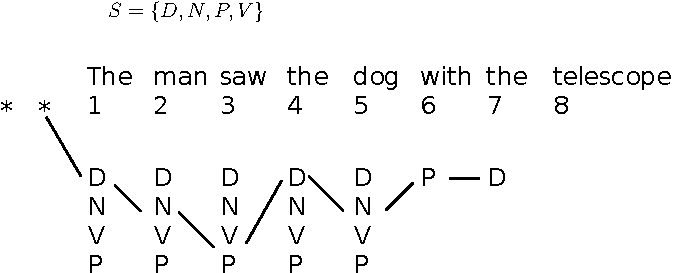
\includegraphics[scale = 0.6]{pics/viterbi1.pdf}
\end{figure}

\begin{itemize}
    \item Hay muchas secuencias posibles de etiquetas.
    \item Cada una de ellas tiene una probabilidad calculada a partir de los parámetros $q$ y $e$.
    \item $\pi(7, P, D)$ es la máxima probabilidad de que una de estas secuencias de etiquetas termine en $P$ y $D$ en la posición $7$.
    \item La ruta representa la secuencia con la máxima probabilidad.
\end{itemize}

\subsection{Una Definición Recursiva}

\textbf{Caso base:}

\[
\pi(0, *, *) = 1
\]

\textbf{Definición recursiva:}

Para cualquier $k \in \{1 \ldots n\}$, para cualquier $u \in S_{k-1}$ y $v \in S_k$:

\[
\pi(k, u, v) = \max_{w \in S_{k-2}} (\pi(k - 1, w, u) \times q(v|w, u) \times e(x_k|v))
\]

\paragraph{Justificación de la Definición Recursiva}

Para cualquier $k \in \{1 \ldots n\}$, para cualquier $u \in S_{k-1}$ y $v \in S_k$:

\[
\pi(k, u, v) = \max_{w \in S_{k-2}} (\pi(k - 1, w, u) \times q(v|w, u) \times e(x_k|v))
\]

\begin{figure}[h]
    \centering
    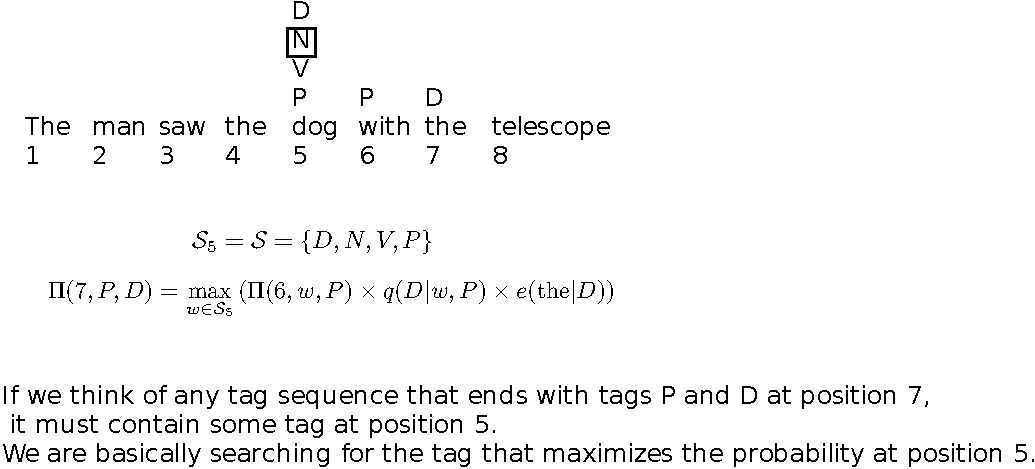
\includegraphics[scale = 0.6]{pics/viterbi2.pdf}
\end{figure}



\begin{itemize}
    \item Consideremos una secuencia de etiquetas arbitraria que termina con las etiquetas $P$ y $D$ en la posición $7$.
    \item Debe contener alguna etiqueta en la posición $5$.
    \item Básicamente, estamos buscando la etiqueta que maximiza la probabilidad en la posición $5$.
\end{itemize}

\subsection{El Algoritmo de Viterbi}

\begin{algorithm}[H]
\SetKwInput{Input}{Entrada}
\SetKwInput{Initialization}{Inicialización}
\SetKwFunction{Max}{max}
\SetKwFunction{Return}{retornar}

\Input{una oración $x_1 \ldots x_n$, parámetros $q(s|u, v)$ y $e(x|s)$}

\Initialization{Establecer $\pi(0, *, *) = 1$;  $S_{-1} = S_0 = \{*\}$, $S_k = S$ para $k \in \{1 \ldots n\}$.
}

\BlankLine
\SetAlgoLined
\caption{Algoritmo de Viterbi}
\label{algo:prob_inference}
\BlankLine

\For{$k = 1$ \KwTo $n$}{
\For{$u \in S_{k-1}, v \in S_k$}{
$\pi(k, u, v) = \max_{w \in S_{k-2}} (\pi(k - 1, w, u) \times q(v|w, u) \times e(x_k|v))$
}
}

\BlankLine
\Return{$\max_{u \in S_{n-1}, v \in S_n} (\pi(n, u, v) \times q(\text{STOP}|u, v))$}
\end{algorithm}

\subsection{El Algoritmo de Viterbi con Punteros de Retroceso}

\begin{algorithm}[H]
\SetKwInput{Input}{Entrada}
\SetKwInput{Initialization}{Inicialización}
\SetKwFunction{Max}{max}
\SetKwFunction{ArgMax}{argmax}
\SetKwFunction{Return}{retornar}

\Input{una oración $x_1 \ldots x_n$, parámetros $q(s|u, v)$ y $e(x|s)$}

\Initialization{Establecer $\pi(0, *, *) = 1$;  $S_{-1} = S_0 = \{*\}$, $S_k = S$ para $k \in \{1 \ldots n\}$.
}

\BlankLine
\SetAlgoLined
\caption{Algoritmo de Viterbi con Punteros de Retroceso}
\label{algo:viterbi}
\BlankLine

\For{$k = 1$ \KwTo $n$}{
\For{$u \in S_{k-1}, v \in S_k$}{
\[
\pi(k, u, v) = \max_{w \in S_{k-2}} (\pi(k - 1, w, u) \times q(v|w, u) \times e(x_k|v))
\]    
\[
\text{bp}(k, u, v) = \arg \max_{w \in S_{k-2}} (\pi(k - 1, w, u) \times q(v|w, u) \times e(x_k|v))
    \]} 
}



\BlankLine
$(y_{n-1}, y_n) = \arg \max_{(u,v)} (\pi(n, u, v) \times q(\text{STOP}|u, v))$ \tcp*[r]{Find maximum probability and corresponding tags}
\For{$k = (n - 2)$ \KwTo $1$}{
$y_k = \text{bp}(k + 2, y_{k+1}, y_{k+2})$ \tcp*[r]{Retrieve tag sequence using backpointers}
}

\BlankLine
\Return{the tag sequence $y_1 \ldots y_n$} \tcp*[r]{Return the final tag sequence}
\end{algorithm}

En el Algoritmo \ref{algo:viterbi}, se utiliza el puntero de retroceso para reconstruir la secuencia de etiquetas con la máxima probabilidad. El algoritmo recorre las tablas $\pi$ en orden inverso, comenzando desde la posición $n$ hasta la posición $1$. En cada iteración, se elige la etiqueta $u$ y $v$ que maximizan la expresión $\pi(k, u, v) \times q(\text{STOP}|u, v)$. Estas etiquetas se agregan al comienzo de la secuencia de etiquetas $path$, y al final del algoritmo, se devuelve la secuencia $path[1:-1]$, eliminando las etiquetas de inicio y detención.

Con el algoritmo de Viterbi, podemos encontrar eficientemente la secuencia de etiquetas más probable para una oración dada, utilizando programación dinámica y aprovechando la estructura de dependencia entre las etiquetas en el HMM. Esto es especialmente útil en problemas de etiquetado de secuencias, como el etiquetado de partes del habla en NLP. 

\subsection{El Algoritmo de Viterbi: Tiempo de Ejecución}
El tiempo de ejecución del algoritmo de Viterbi se puede analizar de la siguiente manera:

\begin{itemize}
    \item Se requiere un tiempo de $O(n|S|^3)$ para calcular $q(s|u, v) \times e(x_k|s)$ para todos los valores de $k, s, u, v$.
    \item La tabla $\pi$ tiene $n|S|^2$ entradas que deben ser llenadas.
    \item Se necesita un tiempo de $O(|S|)$ para llenar una entrada.
\end{itemize}

Por lo tanto, el tiempo de ejecución total es $O(n|S|^3)$.

\paragraph{Ventajas y Desventajas}
El uso de etiquetadores basados en Modelos de Markov Ocultos (HMM) presenta ciertas ventajas y desventajas:

\begin{itemize}
    \item Los etiquetadores HMM son fáciles de entrenar (se recopilan conteos a partir de un corpus de entrenamiento).
    \item Tienen un rendimiento relativamente bueno (más del 90\% de precisión en el reconocimiento de entidades nombradas).
    \item La principal dificultad radica en modelar $e(\text{palabra} | \text{etiqueta})$, lo cual puede ser muy complejo si las "palabras" son complejas.
\end{itemize}

Aunque los etiquetadores HMM tienen ventajas en términos de simplicidad y rendimiento, la modelización de la probabilidad condicional $e(\text{palabra} | \text{etiqueta})$ puede resultar desafiante en situaciones donde las palabras son complejas o ambiguas. En tales casos, se pueden requerir técnicas más avanzadas para mejorar la precisión del etiquetado de secuencias.


\section{MEMMs}  
  
\begin{itemize}

\item Maximum-entropy Markov models (MEMMs) make use of log-linear multi-class models for sequence labeling tasks \cite{mccallum2000maximum}.
 
 \item In the early NLP literature, logistic regression was often called maximum entropy classification \cite{jacobbook}.
 
 \item Hence, MEMMs will look very similar to the multi-class softmax models seen in the lecture about linear models. 
 
  \item In contrast to HMMs, here we rely on parameterized functions.


 \item The goal of MEMMs is  model the following conditional distribution:
 
 \begin{displaymath}
  P(s_1,s_2 \dots, s_m | x_1, \dots, x_m)
 \end{displaymath}

 \item Where each $x_j$ for $j = 1 \dots m$ is the $j$-th input symbol (for example the j-th word in a sentence), and each $s_j$ for $j = 1 \dots m$ is the $j$-th tag.\footnote{These slides are based on lecture notes of Michael Collins \url{http://www.cs.columbia.edu/~mcollins/crf.pdf}. The notation and terminology has been adapted to be consistent with the rest of the course.}

\item We would expect $P$(DET,NOUN,VERB$|$the,dog,barks$)$ to be higher than $P$(VERB,VERB,VERB$|$the,dog,barks$)$ in a model trained from a POS-tagging training dataset.
 
\item We use $S$ to denote the set of possible tags.
\item We assume that $S$ is a finite set. 
 \item For example, in part-of-speech tagging of English, $S$ would be the set of all possible parts of speech in English (noun, verb, determiner, preposition, etc.).
 \item Given a sequence of words $x_1, \dots, x_m$ , there are $k^m$ possible part-of-speech sequences $s_1, \dots, s_m$ , where $k = |S|$ is the number of possible parts of speech.
 \item We want to estimate a distribution over these $k^m$ possible sequences.

 \item In a first step, MEMMs use the following decomposition ($s_0$ has always a special tag $*$):
 \begin{equation}
\begin{split}
  P(s_1,s_2 \dots, s_m | x_1, \dots, x_m) \quad & =  \prod_{i=1}^{m}    P(s_i | s_1 \dots, s_{i-1}, x_1, \dots, x_m)\\
 \quad & =  \prod_{i=1}^{m}    P(s_i | s_{i-1}, x_1, \dots, x_m)
\end{split}
\end{equation}

\item The first equality is exact (it follows by the chain rule of conditional probabilities).

\item The second equality follows from an independence assumption, namely that for all $i$,

\begin{displaymath}
 P(s_i | s_1 \dots, s_{i-1}, x_1, \dots, x_m) =   P(s_i | s_{i-1}, x_1, \dots, x_m)
\end{displaymath}

\item Hence we are making a first order Markov assumption similar to the Markov assumption made in HMMs\footnote{We actually made a second order Markov assumption in HMMs. MEMMs can also be extended to second order assumptions.}. 
 
\item The tag in the $i$-th position depends only on the tag in the $(i -1)$-th position. 
 
 
\item Having made these independence assumptions, we then model each term using a multiclass log-linear (softmax) model:
 
 \begin{equation}
 P(s_i | s_{i-1}, x_1, \dots, x_m)  =  \frac{\exp (\vec{w}\cdot \vec{\phi}(x_1, \cdots, x_m, i, s_{i-1},s_i))}{\sum_{s' \in S} \exp (\vec{w}\cdot \vec{\phi}(x_1, \cdots, x_m, i, s_{i-1},s'))}
\end{equation}
 
\end{itemize}

Here $\vec{\phi}(x_1, \cdots, x_m, i, s_{i-1},s_i)$ is a feature vector where:
\begin{itemize}
 \item $x_1, \cdots, x_m$ is the entire sentence being tagged.
  \item $i$ is the position to be tagged (can take any value from $1$ to $m$).
  \item $s_{i-1}$ is the previous tag value (can take any value in $S$).
  \item $s_i$ is the new tag value (can take any value in $S$).
 
\end{itemize}

The scope of the feature vector is \textbf{restricted} to the whole input sequence $x_1, x_m$, and only the previous and current tag values. This restriction allows efficient training of both MEMMs and CRFs.


\section{Example of Features used in Part-of-Speech Tagging}

\begin{enumerate}
 \item $\vec{\phi}(x_1, \cdots, x_m, i, s_{i-1},s_i)_{[1]}=1$ if $s_i$ = ADVERB and word $x_i$ ends in ``-ly''; 0 otherwise. \\ 
 
 If the weight $\vec{w}_{[1]}$ associated with this feature is large and positive, then this feature is essentially saying that we prefer labelings where words ending in -ly get labeled as ADVERB.
 
 \item $\vec{\phi}(x_1, \cdots, x_m, i, s_{i-1},s_i)_{[2]}=1$ if $i=1$, $s_i$= VERB, and $x_m$=?; 0 otherwise. 
 \\ If the weight $\vec{w}_{[2]}$ associated with this feature is large and positive, then labelings that assign VERB to the first word in a question (e.g., ``Is this a sentence beginning with a verb?'') are preferred.


\item $\vec{\phi}(x_1, \cdots, x_m, i, s_{i-1},s_i)_{[3]}=1$ if $s_{i-1}$= ADJECTIVE and $s_i$= NOUN; 0 otherwise. 
\\Again, a positive weight for this feature means that adjectives tend to be followed by nouns. 

\item $\vec{\phi}(x_1, \cdots, x_m, i, s_{i-1},s_i)_{[4]}=1$ if $s_{i-1}$= PREPOSITION and $s_{i}$= PREPOSITION. 
\\ A negative weight $\vec{w}_{[4]}$ for this function would mean that prepositions don't tend to follow prepositions.

 
\end{enumerate}


\footnotemark{Source: \url{https://blog.echen.me/2012/01/03/introduction-to-conditional-random-fields/}}



\section{Feature Templates}

It is possible to define more general feature templates covering unigrams, bigrams, n-grams of words as well as tag values of $s_{i-1}$ and $s_i$.

\begin{enumerate}
  
 \item A word unigram and tag unigram feature template: $\vec{\phi}(x_1, \cdots, x_m, i, s_{i-1},s_i)_{[index(j,z)]}=1$ if $s_i$ = TAG$_{[j]}$ and $x_i$ = WORD$_{[z]}$; 0 otherwise $\forall j,z$. \\ Notice that $j$ is and index spanning all possible tags in $S$ and $z$ is another index spanning the words in the vocabulary $V$.
 
 \item A word bigram and tag bigram feature template: $\vec{\phi}(x_1, \cdots, x_m, i, s_{i-1},s_i)_{[index(j,z,u,v)]}=1$ if $s_{i-1}$ = TAG$_{[j]}$ and $s_i$ = TAG$_{[z]}$ and $x_{i-1}$ = WORD$_{[u]}$ and $x_{i}$ = WORD$_{[v]}$; 0 otherwise $\forall j,z,u,v$. 
 
 
\end{enumerate}

The function $index(j,k,...)$ will map each different feature to a unique index in the feature vector.  \\
Notice that the resulting vector will be very high-dimensional and sparse.

\paragraph{Example}
  \begin{figure}[h]
        	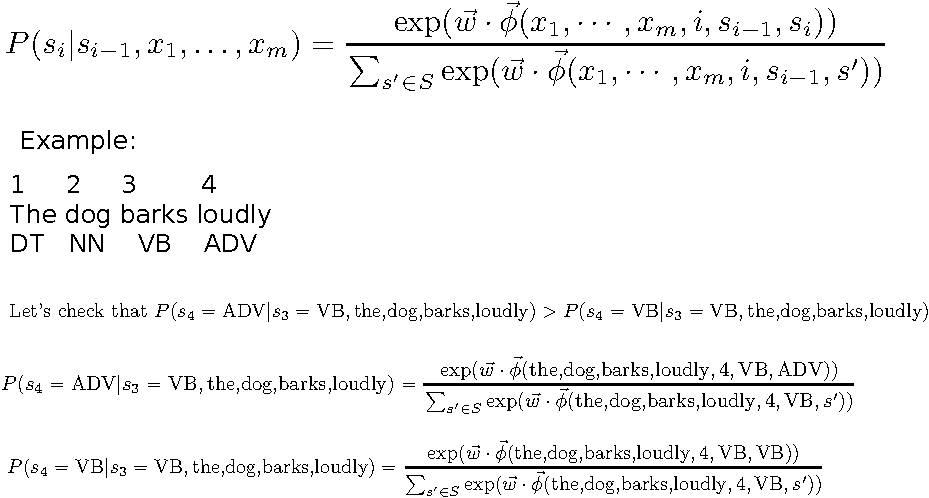
\includegraphics[scale = 0.73]{pics/CRF1.pdf}
        \end{figure}

  \begin{figure}[h]
        	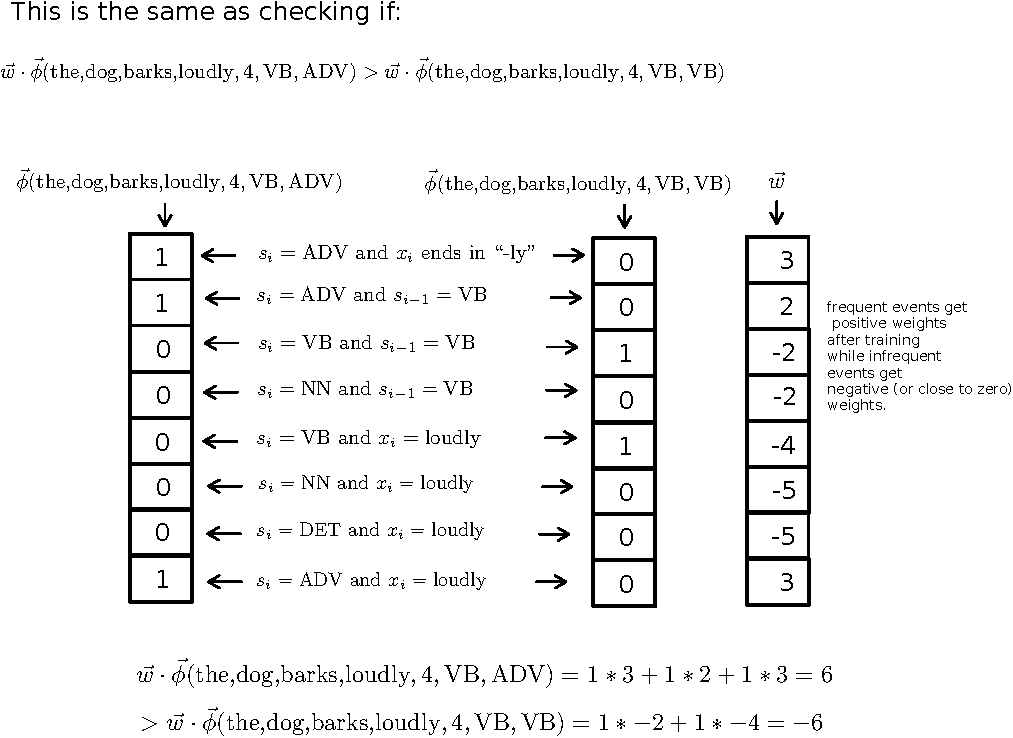
\includegraphics[scale = 0.6]{pics/CRF2.pdf}
        \end{figure}





\section{MEMMs and Multi-class Softmax}

\begin{itemize}
\item Notice that the log-linear model from above is very similar to the multi-class softmax model presented in the lecture about linear models.

\item A general log-linear model has the following form:

\begin{displaymath}
 P( y | x; \vec{w}) = \frac{\exp (\vec{w}\cdot \vec{\phi}(x,y))}{\sum_{y' \in Y} \exp (\vec{w}\cdot \vec{\phi}(x,y'))}
\end{displaymath}


\item A multi-class softmax model has the following form:
\begin{equation}
\begin{split}
\hat{\vec{y}} \quad & =  \operatorname{softmax}(\vec{x} \cdot W + \vec{b})  \\
\hat{\vec{y}}_{[i]} \quad & = \frac{e^{(\vec{x} \cdot W + \vec{b})_{[i]}}}{\sum_j e^{(\vec{x} \cdot W + \vec{b})_{[j]}}}
\end{split}
\end{equation}

 
\item Difference 1: in the log-linear model we have a fixed parameter vector $\vec{w}$ instead of having multiple vectors (one column of $W$ for each class value).

\item Difference 2: the feature vector of the log-linear model $\vec{\phi}(x,y)$ includes information of the label $y$, whereas the input vector $\vec{x}$ of the softmax model is independent of $y$. 

\item Log-linear models allow using features that consider the interaction between $x$ and $y$ (e.g., $x$ ends in ``ly'' and $y$ is an ADVERB).

 
\end{itemize}



\section{Training MEMMs}

\begin{itemize}

\item Once we've defined the feature vectors $\vec{\phi}$, we can train the parameters $\vec{w}$ of the model in the usual way linear models are trained.

\item We set the negative log-likelihood as the loss function and optimize parameters using gradient descent from the training examples.

\item This is equivalent as using the cross-entropy loss.

\item ``Any loss consisting of a negative log-likelihood is a cross-entropy between the empirical distribution defined by the training set and the probability distribution defined by model'' \cite{goodfellow2016deep}.  
 
\end{itemize}


\section{Decoding with MEMMs}

\begin{itemize}

\item The decoding problem is as follows.
\item We are given a new test sequence $x_1, \dots, x_m$.
\item Our goal is to compute the most likely state sequence for this test sequence,

\begin{equation}
 \operatorname{arg} \max_{s_1,\dots,s_m} P(s_1,\dots,s_m|x_1,\dots,x_m).
\end{equation}

\item There are $k^m$ possible state sequences, so for any reasonably large sentence length $m$ brute-force search through all the possibilities will not be possible.

\item We can use the Viterbi alogrithm in a similar way as used for HMMs.
 
\item The basic data structure in the algorithm will be a dynamic programming table $\pi$ with entries $\pi[j,s]$ for $j=1, \dots, m$, and $s \in S$.

\item  $\pi[j,s]$ will store the maximum probability for any state sequence ending in state $s$ at position $j$.

\item More formally, our algorithm will compute 
\begin{displaymath}
\pi[j,s] =  \max_{s_1,\dots, s_{j-1}}\left(P(s | s_{j-1}, x_1, \dots, x_m) \prod_{k=1}^{j-1}    P(s_k | s_{k-1}, x_1, \dots, x_m)\right)
\end{displaymath}
for all $j = 1, \dots,m$, and for all $s \in S$.

\end{itemize}

The algorithm is as follows:

\begin{itemize}

\item  Initialization: for $s \in  S$

\begin{displaymath}
  \pi[1,s] = P (s | s_0,x_1,\dots,x_m)
\end{displaymath}
where $s_0$ is a special ``initial'' state.

\item For $j \in \{2,\dots,m\}$, $s \in  \{1,\dots,k\}$

\begin{displaymath}
  \pi[j,s] =  \max_{s' \in S} \ [\pi[j-1,s'] \times P (s | s',x_1,\dots,x_m)]
\end{displaymath}


\item  Finally, having filled in the $\pi[j,s]$ values for all $j, s$, we can calculate

\begin{displaymath}
  \max_{s_1,\dots,s_m} = \max_{s} \ \pi[m,s].
\end{displaymath}


\item The algorithm runs in $O(mk^2)$ time (i.e., linear in the sequence length $m$,
and quadratic in the number of tags $k$).


\item As in the Viterbi algorithm for HMMs, we can compute the highest-scoring sequence using backpointers in the dynamic programming algorithm.

\end{itemize}




\section{Comparison between MEMMs and HMMs}

\begin{itemize}

\item  So what is the motivation for using MEMMs instead of HMMs?

\item Note that the Viterbi decoding algorithms for the two models are very similar. 

\item In MEMMs, the probability associated with each state transition $s_{i-1}$ to $s_i$ is

 \begin{displaymath}
 P(s_i | s_{i-1}, x_1, \dots, x_m)  =  \frac{\exp (\vec{w}\cdot \vec{\phi}(x_1, \cdots, x_m, i, s_{i-1},s_i))}{\sum_{s' \in S} \exp (\vec{w}\cdot \vec{\phi}(x_1, \cdots, x_m, i, s_{i-1},s'))}
\end{displaymath}


\item In HMMs, the probability associated with each transition is:

\begin{displaymath}
 P(s_i | s_{i-1}, x_1, \dots, x_m) = P(s_1|s_{i-1})P(x_i|s_i)
\end{displaymath}

\item  The key advantage of MEMMs is that the use of feature vectors $\vec{\phi}$ allows much
richer representations than those used in HMMs.

\item For example, the transition probability can be sensitive to any word in the input sequence $x_1, \dots, x_m$.

\item In addition, it is very easy to introduce features that are sensitive to spelling features (e.g., prefixes or suffixes) of the current word $x_i$, or of the surrounding words.

\item These features are useful in many NLP applications, and are difficult to incorporate within HMMs in a clean way.

\end{itemize}



\section{Conditional Random Fields (CRFs)}


\begin{itemize}

\item  We now turn to Conditional Random Fields (CRFs) \cite{LaffertyMP01}.

\item Notation: for convenience, we'll use $x_{1:m}$ to refer to an input sequence $x_1 ,\dots,x_m$, and $s_{1:m}$ to refer to a sequence of tags $s_1, \dots, s_m$.

\item The set of all possible tags is again $S$.

\item The set of all possible tag sequences is $S^m$.

\item In conditional random fields we'll again build a model of
\begin{displaymath}
 P(s_1, \dots, s_m | x_1, \dots, x_m) = P(s_{1:m}|x_{1:m})
\end{displaymath}


\item A first key idea in CRFs will be to define a feature vector  that maps an entire input sequence $x_{1:m}$ paired with an entire tag sequence $s_{1:m}$ to some $d$-dimensional feature vector:

\begin{displaymath}
 \vec{\Phi}(x_{1:m},s_{1:m}) \in \mathcal{R}^d
\end{displaymath}

\item We'll soon give a concrete definition for $\vec{\Phi}$.
\item  For now just assume that some definition exists. 
\item We will often refer to $\vec{\Phi}$ as being a ``global'' feature vector.
\item It is global in the sense that it takes the entire state
sequence into account.

\item item In CRFs we build a giant log-linear model:

\begin{displaymath}
 P(s_{1:m}|x_{1:m}; \vec{w}) = \frac{\exp (\vec{w} \cdot \vec{\Phi}(x_{1:m},s_{1:m}))}{\sum_{s'_{1:m} \in S^m}\exp (\vec{w} \cdot \vec{\Phi}(x_{1:m},s'_{1:m}))}
\end{displaymath}

\item This is ``just'' another log-linear model, but it is ``giant''.
\item The space of possible values for $s_{1:m}$ is huge $S^m$. 
\item The normalization constant (denominator in the above expression) involves a sum over all possible tag sequences $S^m$.
\item These issues might seem to cause severe computational problems.
\item  Under appropriate assumptions we can train and decode efficiently
with this type of model.
\item  We define the global feature vector $\vec{\Phi}(x_{1:m},s_{1:m})$ as follows: 

\begin{displaymath}
 \vec{\Phi}(x_{1:m},s_{1:m}) = \sum_{j=1}^{m} \vec{\phi}(x_{1:m},j,s_{j-1},s_j) 
\end{displaymath}

where $\vec{\phi}(x_{1:m},j,s_{j-1},s_j)$ are the same as the feature vectors used in MEMMs.

\item  Example: \ $ \vec{\Phi}([\text{the,dog,barks}],\text{DET,NOUN,VERB}]) = \vec{\phi}([\text{the,dog,barks}],1,*,\text{DET}) + \vec{\phi}([\text{the,dog,barks}],2,\text{DET},\text{NOUN}) + \vec{\phi}([\text{the,dog,barks}],3,\text{NOUN},\text{VERB})$

\item Essentially, we are adding up many sparse vectors.



\end{itemize}


\paragraph{Example}
  \begin{figure}[h]
        	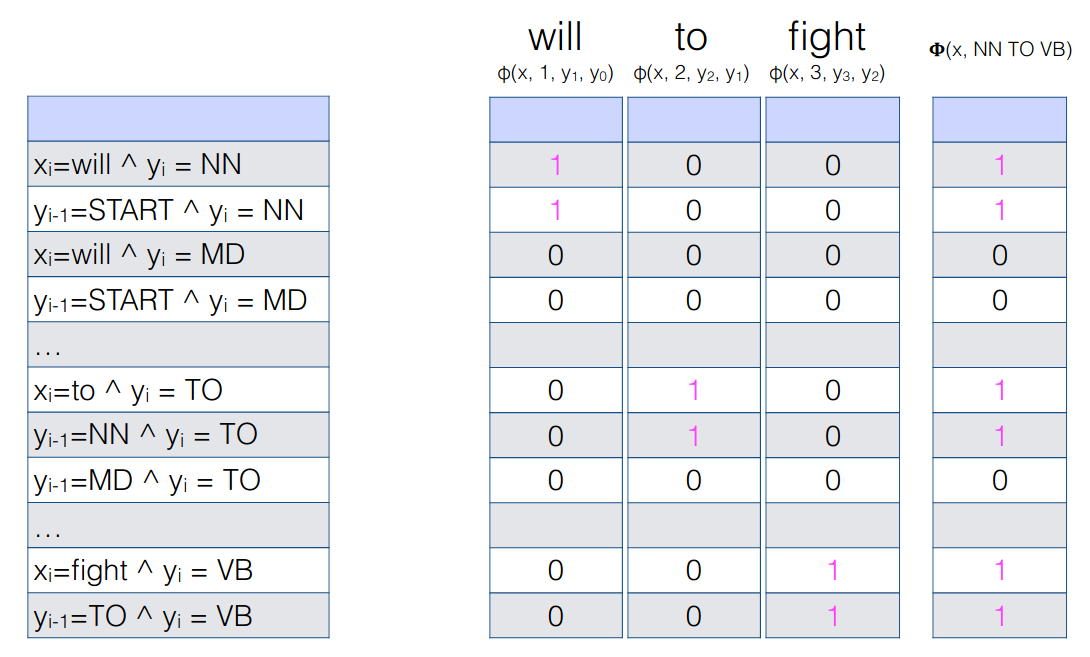
\includegraphics[scale = 0.26]{pics/CRF3.png}
        \end{figure}
        
        \footnotemark{source: \url{http://people.ischool.berkeley.edu/~dbamman/nlpF18/slides/12_neural_sequence_labeling.pdf}}


\begin{itemize}
\item We are assuming that for any dimension of $\vec{\Phi}_{[k]}, k= 1, \dots, d$, the $k$'th global feature is:

\begin{displaymath}
 \vec{\Phi}(x_{1:m},s_{1:m})_{[k]} = \sum_{j=1}^{m} \vec{\phi}(x_{1:m},j,s_{j-1},s_j)_{[k]} 
\end{displaymath}

\item Thus $\vec{\Phi}(x_{1:m},s_{1:m})_{[k]}$ is calculated by summing the ``local'' feature vector $\vec{\phi}(x_{1:m},j,s_{j-1},s_j)_{[k]}$  over the m different tag transitions in $s_1,\dots,s_m$.


\item We would expect each local vector to encode relevant information about the tag transition by turning on some vector dimensions (setting the value to one).

\item We now turn to two critical practical issues in CRFs: first, decoding, and sec-
ond, parameter estimation (training).

\end{itemize}




\section{Decoding with CRFs}

\begin{itemize}
\item The decoding problem in CRFs is as follows.
\item For a given input sequence $x_{1:m} = x_1 , x_2 , \dots, x_m$ , we would like to find the most likely underlying  state sequence under the model, that is,

\begin{equation}
 \begin{split}
 arg \max_{s_{1:m} \in S^m} P(s_{1:m}| x_{1:m}; \vec{w})  \quad & =  arg \max_{s_{1:m} \in S^m} \frac{\exp (\vec{w} \cdot \vec{\Phi}(x_{1:m},s_{1:m}))}{\sum_{s'_{1:m} \in S^m}\exp (\vec{w} \cdot \vec{\Phi}(x_{1:m},s'_{1:m}))} \\
 \quad & =  arg \max_{s_{1:m} \in S^m} \exp (\vec{w} \cdot \vec{\Phi}(x_{1:m},s_{1:m})) \\
  \quad & =  arg \max_{s_{1:m} \in S^m}  \vec{w} \cdot \vec{\Phi}(x_{1:m},s_{1:m}) \\
    \quad & =  arg \max_{s_{1:m} \in S^m}  \vec{w} \cdot \sum_{j=1}^{m} \vec{\phi}(x_{1:m},j,s_{j-1},s_j) \\
 \quad & =  arg \max_{s_{1:m} \in S^m}  \sum_{j=1}^{m} \vec{w} \cdot \vec{\phi}(x_{1:m},j,s_{j-1},s_j)   
 \end{split}
 \end{equation}

\item We have shown that finding the most likely sequence under the model is equivalent to finding the sequence that maximizes:

\begin{displaymath}
 arg \max_{s_{1:m} \in S^m}  \sum_{j=1}^{m} \vec{w} \cdot \vec{\phi}(x_{1:m},j,s_{j-1},s_j)  
\end{displaymath}

\item This problem has a clear intuition. Each transition from tag  $s_{j-1}$ to tag $s_j$ has an associated score:  $\vec{w} \cdot \vec{\phi}(x_{1:m},j,s_{j-1},s_j)$  


\item This score could be positive or negative. 

\item Intuitively, this score will be relatively high if the state transition is plausible, relatively low if this transition is implausible.

\item  The decoding problem is to find an entire sequence of states such that the sum of transition scores is maximized.

\item We can again solve this problem using a variant of the Viterbi algorithm, in a very similar way to the decoding algorithm for HMMs or MEMMs.

\end{itemize}


\section{Parameter Estimation in CRFs (training)}


\begin{itemize}
\item For parameter estimation, we assume we have a set of $n$ labeled examples, $\{(x_{1:m}^i, s_{1:m}^i )\}_{i=1}^n$ . Each $x_{1:m}^i$ is an input sequence $x_1^i, \dots , x_m^i$ each $s_{1:m}^i$ is a tag sequence $s_1^i, \dots , s_m^i$.

\item We again set the negative log-likelihood (or cross-entropy) as the loss function $L$ as optimize parameters using gradient descent.

\item The main challenge here is that gradient calculations $\frac{\partial L}{\partial \vec{w}_{[k]}}$ involve summing over $S^m$ (a very large set containing all possible tag sequences).

\item This sum can be computed efficiently using the Forward-backward algorithm\footnote{\url{http://www.cs.columbia.edu/~mcollins/fb.pdf}}. 

\item This is another dynamic programming algorithm that is closely related
to the Viterbi algorithm.

\end{itemize}



\section{CRFs and MEMMs}

\begin{itemize}

\item CRFs and MEMMS are discriminative sequence labeling models: they model the conditional probability directly via a parameterized log-linear multi-class function (softmax).

\item HMMs, on the other hand, are generative models.

\item In MEMM the normalization (denominator of the softmax) is local: it happens at each tag step (the sum runs over all possible tag values $S$).

\item In CRFs the normalization is global: the sum runs over all possible tag sequences $S^m$.

\item Training a MEMM is quite easy: just train a multi-class log-linear model for for a given word to the label. This classifier is used at each word step to predict the whole sequence.

\item Training CRF is more complex. The objective  is to maximize the log probability of the most likely sequence.


\end{itemize}






\subsection{CRFs and MEMMs: the label bias problem}

\begin{itemize}

\item MEMMs end up making up decision at each time step independently.

\item This leads to a problem called label bias: in some tag space configurations, MEMMs essentially completely ignore important aspects of the context.

\item Example: The right POS labeling of sentence ``will to fight'' (la voluntad de pelear) is ``NN TO VB''. \footnote{Here we are using the PENN Treebank tagset: \url{https://www.eecis.udel.edu/~vijay/cis889/ie/pos-set.pdf}} 

\item Here NN stands for ``noun'', TO stands for ``infinitive to'',  and VB stands for ``verb base form''.

\item Modals (MD) show up much more frequently at the start of the sentence than nouns do (e.g., questions).

\item Hence, tag ``MD'' will receive a higher score than tag ``NN'' when $x_0$=``will'' : $P(s_1 = MD|s_{0} = *,x_1 = \text{``will''},...) > P( s_1 = NN| s_{i-1} = *, x_1 = \text{``will''})$.


\item But we know that MD + TO is very rare: ``... can to eat'', ``... would to eat''.


\item The word ``to'' is relatively deterministic (almost always has tag TO) so it doesn't matter what tag precedes it.

\item Because of the local normalization of MEMMs, $P(s_i = TO | s_{i-1}, x_1, \dots, x_i = \text{``to''}, \dots, x_n)$ will always be 1 when $x_i=$``to'' regardless of the value of $s_{i-1}$ (MD or NN).

\item That means our prediction for ``to'' can't help us disambiguate ``will''.  

\item We lose the information that MD + TO sequences rarely happen.

\item As a consequence: a MEMMS would likely label the first word to ``MD''.

\item CRF overcomes this issue by doing a global normalization: it considers the score of the whole sequence before normalizing to make it a probability distribution.



\end{itemize}



Label Bias
In some state space configurations,MEMMs essentially completely ignore the inputs.
``label bias problem,'' where states with low-entropy transition distributions ``effectively ignore'' their observations.
These are names for situations when one source of information is ignored because it isexplained away by anothersource


\section{Links}

\begin{itemize}

\item \url{http://people.ischool.berkeley.edu/~dbamman/nlpF18/slides/11_memm_crf.pdf}

\item \url{http://people.ischool.berkeley.edu/~dbamman/nlpF18/slides/12_neural_sequence_labeling.pdf}

\item \url{https://www.depends-on-the-definition.com/sequence-tagging-lstm-crf/}

\item \url{https://www.quora.com/What-are-the-pros-and-cons-of-these-three-sequence-models-MaxEnt-Markov-Model-Conditional-random-fields-and-recurrent-neural-networks}

\item \url{https://people.cs.umass.edu/~mccallum/papers/crf-tutorial.pdf}

\item \url{http://www.davidsbatista.net/blog/2017/11/13/Conditional_Random_Fields} 

\end{itemize}

  
